\begin{frame}{Gestión documental de titulación: dónde usamos servicios web}
{\small Estudiantes, directores y tribunal trabajan el documento de titulación en la web: lo escriben, lo revisan, lo aprueban y descargan el expediente en PDF.\par}
{\scriptsize\color{gris}Repositorio: \texttt{Troyano2004/sistema-titulacion-uteq}\par}
\vspace{10pt}
\centering
\begin{tikzpicture}[node distance=0.9cm and 2.2cm, caja/.style={draw=verde,rounded corners=3pt,fill=verdesuave,minimum width=2.6cm,minimum height=0.9cm,font=\small,align=center}, flecha/.style={-{Stealth[length=2.5mm]},thick,color=tinta}, etiqueta/.style={font=\scriptsize,color=gris}]
\node[caja] (front) {Angular\\{\scriptsize navegador}};
\node[caja,right=of front] (back) {Spring Boot 4\\{\scriptsize API REST}};
\node[caja,right=of back] (bd) {PostgreSQL};
\node[caja,below=of back] (arch) {Azure Blob Storage\\{\scriptsize PDF de los documentos}};
\draw[flecha] (front) -- node[above,etiqueta]{REST / JSON} (back);
\draw[flecha] (back) -- node[above,etiqueta]{JPA} (bd);
\draw[flecha] (back) -- node[right,etiqueta]{multipart} (arch);
\end{tikzpicture}
\par\vspace{8pt}
\begin{columns}[T]
\begin{column}{0.4\textwidth}
\cifra{67}{controladores REST}
\end{column}
\begin{column}{0.4\textwidth}
\cifra{396}{\emph{endpoints}}
\end{column}
\end{columns}
\end{frame}

\begin{frame}{Recursos y verbos HTTP}
\centering
\footnotesize
\begin{tabular}{@{}lllc@{}}
\toprule
Método & URI & Qué hace & Idempotente \\
\midrule
\texttt{GET} & \texttt{/documento/\{id\}} & Consulta el documento & Sí \\
\texttt{GET} & \texttt{/documento/\{id\}/observaciones} & Lista observaciones & Sí \\
\texttt{PUT} & \texttt{/estudiante/\{id\}/documento} & Guarda cambios & Sí \\
\texttt{POST} & \texttt{/director/\{id\}/documento/\{id\}/observacion} & Crea una observación & \textcolor{rojo}{No} \\
\bottomrule
\end{tabular}
\par\vspace{2pt}
{\scriptsize\color{gris} Prefijo: \texttt{/api/titulacion2}\par}
\vspace{10pt}
\begin{block}{Por qué importa}
Si repito el \texttt{PUT}, el documento queda igual. Si repito el \texttt{POST}, el director deja dos observaciones. Solo el primero se puede reintentar sin miedo.
\end{block}
\fuente{rfc9110}
\end{frame}

\begin{frame}{Una petición real y lo que mejoré}
{\small\texttt{GET /api/titulacion2/documento/\{id\}}\par}
\vspace{4pt}
\begin{columns}[c]
\begin{column}{0.64\textwidth}
\centering
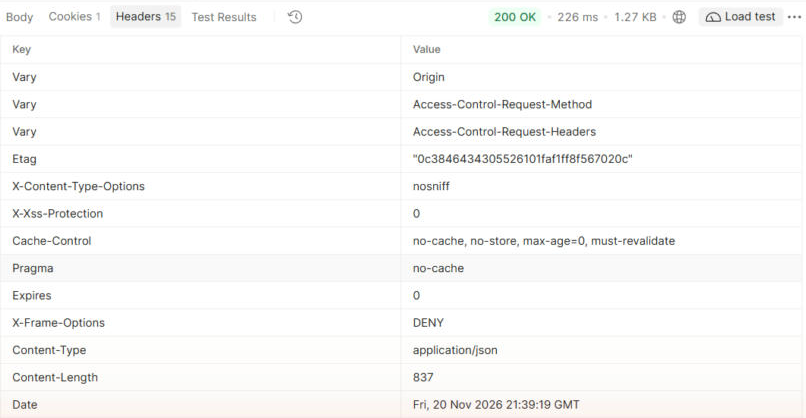
\includegraphics[width=\linewidth,height=4.0cm,keepaspectratio]{../figuras/rivas-peticion.png}
\end{column}
\begin{column}{0.33\textwidth}
\small
\begin{itemize}
\item \texttt{200 OK}, o \texttt{404} si no existe
\item \texttt{Content-Type: application/json}
\item \texttt{ETag}: con \texttt{If-None-Match} responde \texttt{304}
\end{itemize}
\end{column}
\end{columns}
\vspace{2pt}
\begin{alertblock}{Cambios en mi API}
Antes un documento inexistente daba \texttt{500}; ahora da \texttt{404}. Crear una observación devuelve \texttt{201 Created}. El documento lleva \texttt{ETag}. Commit \texttt{d816355}.
\end{alertblock}
\fuente{rfc9110}
\end{frame}
